\documentclass[11pt,letterpaper]{article}
\usepackage[margin=2cm,includefoot]{geometry}
\usepackage[spanish]{babel}

\usepackage{csquotes}
\usepackage{multicol}

\usepackage{qtree}

\usepackage{amsmath}
\usepackage{amsthm}
\usepackage{amssymb}
\usepackage{listings}

\usepackage{enumerate}
\usepackage{tikz}
\usepackage{multicol}
\graphicspath{ {images/} }

\title{\large{Ronda de rescate}}
\author{Diego Méndez Medina}
\date{}
\begin{document}
\maketitle

Me fue bien en los examenes, pero al final del semestre me dio covid y
no pude hacer el ultimo semanal. Hago estas cinco preguntas esperando
suplan la del semanal.

\begin{enumerate}
  %% 01
\item Dada una fŕrmula de la lógica proposicional $\varphi$, se define
  su fórmula complementaria, denotadacomo $\varphi^c$, como el resultado
  de sustituir en $\varphi$ cada presencia de las variables proposicionales
  por su negación. Por ejemplo para la fórmula $p\lor q$ su complementaria
  es $\neg p \lor \neg q$.
  \begin{enumerate}
    %% 01.a
  \item Da la definición recursiva de una función \texttt{fcomp} que recibe
    una fórmula de la lógica proposicional y regresa su complementaria.
    \ttfamily

    \begin{align*}
      \text{fcomp} &: LPROP \rightarrow LPROP\\
      \text{fcomp} (\bot) &= \bot
      & &\text{$\bot$ es una constante, no es una variable}\\
      \text{fcomp}(\top) &= \top
      & &\text{$\top$ es una constante, no es una variable}\\
    \text{fcomp} (p) &= \neg p & &\text{Si $p$ es variable prop}\\
    \text{fcomp} (\neg\varphi) &= \neg \text{fcomp}(\varphi)\\
    \text{fcomp} (\varphi\lor\psi) &=
    \text{fcomp}(\varphi)\lor\text{fcomp}(\psi)\\
    \text{fcomp} (\varphi\land\psi) &=
    \text{fcomp}(\varphi)\land\text{fcomp}(\psi)\\
    \text{fcomp} (\varphi\rightarrow\psi) &=
    \text{fcomp}(\varphi)\rightarrow\text{fcomp}(\psi)\\
    \text{fcomp} (\varphi\leftrightarrow\psi) &=
    \text{fcomp}(\varphi)\leftrightarrow\text{fcomp}(\psi)\\
    \end{align*}

    \rmfamily
    %% 01.b
  \item Demuestra que si $\models \varphi$  entonces $\models \varphi^c$.
  \end{enumerate}

  %% 02
\item Considera el siguiente argumento lógico:
  
  {\it Si mi cliente es culpable, entonces el cuchillo estaba en el cajón. El
  cuchillo no estaba en el cajón o Juan Pablo escondió el cuchillo. No es
  cierto que, si encontraron el cuchillo el $10$ de Septiembre entonces
  Juan Pablo escondió el cuchillo. Además, si no encontraron el cuchillo el
  $10$ de Septiembre, entonces el cuchillo estaba en el cajón y el martillo
  estaba en el establo. Pero sabemos que el martillo no estaba en el
  establo. Por lo tanto mi cliente es inocente.}
  \begin{enumerate}
    %% 02.a
  \item Traduce el argumento anterior a lógica preposicional, indicando
    el glosario empleado.

    Consideramos el siguiente glosario:

    \begin{align*}
      p&:\text{Mi cliente es culpable}\\
      q&:\text{El cuchillo estaba en el cajón}\\
      r&:\text{Juan Pablo escondió el cuchillo}\\
      s&:\text{Encontraron el cuchillo el $10$ de Septiembre.}\\
      t&:\text{El martillo estaba en el establo.}
    \end{align*}

    Tenemos el siguiente argumento:
    \begin{itemize}
    \item[] $p\rightarrow q$
    \item[] $\neg q\lor r$
    \item[] $\neg(s\rightarrow r)$
    \item[] $\neg s\rightarrow (q\land t)$
    \item[] $\neg t$\\
      \rule{.3\textwidth}{0.2mm}
    \item[] $\therefore \neg p$
    \end{itemize}
    %% 02.b
  \item Decide si el argumento es correcto o no. Indica qué método
    vas a utilizar para decidirlo.

    Vamos a resolver con resolución binaria.
    Pasando el argumento a forma normal conjuntiva:
    \begin{itemize}
    \item[] $fnc(p\rightarrow q) = \neg p\lor q$
    \item[] $fnc(\neg q\lor r) = \neg q\lor r$
    \item[] $fnc(\neg(s\rightarrow r)) = \neg(\neg s\lor r) = s\land \neg r$
    \item[] $fnc(\neg s\rightarrow (q\land t)) \equiv s\lor (q\land t)
      = (s\land q) \lor (s\land t)$
    \item[] $fnc(\neg t) = \neg t$\\
      \rule{.3\textwidth}{0.2mm}
    \item[] $\therefore \neg p$
    \end{itemize}
  \end{enumerate}

  Sea $\sigma = \{\neg p\lor q,\neg q\lor r,s\land \neg r,
  (s\land q) \lor (s\land t), \neg t\}$,
  las premisas del argumento dado, queremos ver si:
  $$ \sigma \models \neg p$$

  Basta demostrar que $\sigma\cup \{p\}$ es insatisfasible. Procedemos
  a hacerlo:
  \begin{align*}
    1.&\  \neg p\lor q& &\text{Hip.} \\
    2.&\ \neg q\lor r& &\text{Hip.}\\
    3.&\  s\land \neg r& &\text{Hip.}\\
    4.&\  (s\land q) \lor (s\land t)& &\text{Hip.}\\
    5.&\ \neg t & &\text{Hip.}\\
    6.&\ p & &\text{Hip.}\\
    7.&\ s\land q & &\text{Res}(4,5)\\
    8.&\ \neg r & &\text{Por 3.}\\
    9.&\ q & &\text{Por 7.}\\
    10.&\ r& &\text{Res}(2,9)\\
    11.&\ \square& &\text{Res}(8,10)\\
  \end{align*}
  %% 04
\item[4.] Considera la siguiente fórmula $A$:
  $$ A =_{def} (\forall x\exists z(\neg P(x) \rightarrow T(y, z))[y := a][z := x]
  \land \forall v(\exists xR(v, x, y) \land P(x)))[x, y := f(w), g(v)]$$
  \begin{enumerate}
  \item Determina el alcance de cada uno de los cuantificadores de
    $A$ antes de realizar las sustituciones.

    Los cuantificadores $\forall x\exists z$
    tienen como alcance $\neg P(x) \rightarrow T(y, z)$.

    El cuantificador $\forall v$ tiene como alcance
    $\exists xR(v, x, y) \land P(x)$.

    Por último el cuantificador $\exists x$ tiene como
    alcance $R(v, x, y)$.
  \item Obtén el conjunto de variables libres de $A$ antes de realizar
    las sustituciones.

    $y$ figura libre en $\neg P(x) \rightarrow T(y, z)$.

    $y$ figura libre tambíen en $R(v, x, y)$.

    $x$ figura libre en $P(x)$.

    $$FV(A) = \{y,x\}$$
  \item Realiza las sustituciones indicadas para obtener una fórmula $B$,
    indicando explícitamente los pasos realizados de acuerdo al algoritmo
    de sustitución visto en clase.

    \begin{align*}
      \forall x\exists z(\neg P(x) \rightarrow T(y, z))[y := a][z := x]
      \land \forall v(\exists xR(v, x, y) \land P(x))[x, y := f(w), g(v)]
      &\equiv_\alpha\\
      \forall x\exists w(\neg P(x) \rightarrow T(y, w))[y := a][z := x]
      \land \forall v(\exists uR(v, u, y) \land P(x))[x, y := f(w), g(v)]
      &\equiv\\
      \forall x\exists w(\neg P(x)[y := a][z := x]
      \rightarrow T(y, w)[y := a][z := x])
      \land \forall v(\exists uR(v, u, y) \land P(x))[x, y := f(w), g(v)]
      &\equiv\\
      \forall x\exists w(\neg P(x)
      \rightarrow T(a, w))
      \land \forall v(\exists uR(v, u, y)[x, y := f(w), g(v)]
      \land P(x)[x, y := f(w), g(v)])
      &\equiv\\
      \forall x\exists w(\neg P(x)
      \rightarrow T(a, w))
      \land \forall v(\exists uR(v, u, g(v))
      \land P(f(w))
    \end{align*}
  \item Construye el árbol de sintaxis abstracta de la expresión $B$
    resultante del inciso anterior.
    \Tree[.$\land$ [
        [.$\forall x$ [.$\exists w$ [.$\rightarrow$ [.$\neg$ [.$P(x)$ ]]
              [.$T(a,w)$ ]]]]
            [.$\forall v$ [.$\land$ [.$\exists u$ [.$R(v,u,g(v))$ ]][.$P(f(w))$ ]]]]]
  \end{enumerate}
  %% 05
\item[5.] Sea $\mathcal{I} = \{P^(3), Q^(2), f^(1)\}$ y $\mathcal{M} =
  <M, \mathcal{I}>$ donde $M = \{a, b, c\}$ y
  \begin{align*}
  P^\mathcal{I} &= \{(a, a, a),(b, b, b),(b, a, b)\}\\
  Q^\mathcal{I} &= \{(a, a),(b, c),(c, a)\}\\
  f^\mathcal{I}(a) &= a, f^\mathcal{I}(b) = c, f^\mathcal{I}(c) = a
  \end{align*}

  \begin{enumerate}
  \item Decide si $\mathcal{M} \models_\sigma \forall x(Qxfx \land \exists x
    (P ayfx \lor P byfx))$ donde $\sigma(y) = a$

    Lo que em realidad queremos ver es si:
    \begin{align*}
      \mathcal{M} &\models \forall x(Qxfx \land \exists x
      (P aafx \lor P bafx))\\
      \mathcal{M} &\models \forall x (Qxfx \land \exists y
      (P aafy \lor P bafy))\\
      \mathcal{M} &\models \forall x Qxfx \land \exists y
      (P aafy \lor P bafy)\\
    \end{align*}
    Primero veremos que
    $$ \mathcal{M} \models \forall x Qxfx$$
    Checamos los elementos del universo:
    \begin{itemize}
    \item Para $x= a$
      \begin{align*}
        Qafa &=_\mathcal{I} Qaa \in Q^\mathcal{I}
      \end{align*}
    \item Para $x= b$
      \begin{align*}
        Qbfb &=_\mathcal{I} Qbc \in Q^\mathcal{I}
      \end{align*}
    \item Para $x= c$
      \begin{align*}
        Qcfc &=_\mathcal{I} Qca \in Q^\mathcal{I}
      \end{align*}
    \end{itemize}
    Entonces en efecto
    $$ \mathcal{M} \models \forall x Qxfx$$

    Ahora falta ver que:
    $$ \mathcal{M} \models \exists y (P aafy \lor P bafy)$$
    Para $y=a$ tenemos:
    $$ Paafa = Paaa \in P^\mathcal{I}$$

    Concluimos que $\mathcal{M} \models_\sigma \forall x(Qxfx \land \exists x
    (P ayfx \lor P byfx))$ donde $\sigma(y) = a$

    \hfill\break
    %% b
  \item Define un estado $\sigma$ tal que
    $\mathcal{M} \not\models_\sigma \exists x(\neg Qxx) \land P yfyffy
    \rightarrow Qxy \lor Qyfx$

    Primero hacemos una observación:
    $$\exists x(\neg Qxx) \land P yfyffy \rightarrow Qxy \lor Qyfx
    \equiv \exists x(\neg Qxx) \land P yfyffy \rightarrow Qzy \lor Qyfz$$
    
    Entonces hay que ver un estado $\sigma$ tal que
    $\mathcal{M} \not\models_\sigma \exists x(\neg Qxx) \land P yfyffy
    \rightarrow Qzy \lor Qyfz$

    $\sigma$ es tal que:
    \begin{align*}
      \sigma(y) &= a\\
      \sigma(z) &= b
    \end{align*}

    Así el antecedente de la implicación es verdadero pero
    el lado derecho es falso. Veamos por que:
    $$\mathcal{M}\models_\sigma \exists x(\neg Qxx)$$
    Pues para $x = b$ tenemos $Qbb\notin Q^\mathcal{I}$.
    $$\mathcal{M}\models_\sigma Pyfyffy$$
    \begin{align*}
      Pyfyffy &=_\sigma Pafaffa = Paafa = Paaa \in P^\mathcal{I}.
    \end{align*}

    Y ahora veremos que
    $$\mathcal{M} \not\models_\sigma  Qzy \lor Qyfz$$

    \begin{align*}
      Qzy &=_\sigma Q ba \notin Q^\mathcal{I}\\
      Qyfz &=_\sigma Q afb = Qac \notin Q^\mathcal{I}\\
    \end{align*}

    Entonces para la $\sigma$ dada     $\mathcal{M} \not\models_\sigma \exists x(\neg Qxx) \land P yfyffy
    \rightarrow Qxy \lor Qyfx$
    %% c
  \item  Decide si $\mathcal{M} \models \exists x(P xxx \land Qxfx \land\neg Qxx)$
    
    Es cierto pues para $x=b$ tenemos:
    \begin{align*}
      P bbb &\in P^\mathcal{I}\\
      Qbfb = Qbc &\in Q^\mathcal{I} \\
      Qbb &\not\in Q^\mathcal{I}
    \end{align*}
  \end{enumerate}
  %% 09
\item[9.] Considera el siguiente programa lógico.

  \ttfamily
  p\ ([\;],R).
  
  p\ ([H|T1],\,[H|T2])\ :-\ p\ (T1,T2).
  \rmfamily

  \begin{enumerate}
  \item Da una especificación informal del predicado {\tt p}.

    {\tt p} solo regresa {\tt true} si se itera sobre la lista izquierda
    hasta llegar a la lista vacía.

    Y por el segundo enunciado sabemos que {\tt p} solo continua iterando
    ambas listas si la cabeza de ambas listas son iguales.

    \hfill\break
    {\tt p} indica si toda la primera lista recibida es sublista de la segunda
    lista recibida. 
  \item Construye el árbol de búsqueda para la meta {\tt ?- p(X,[1,2,3]}.

    \hfill\break
    
    No se poner las sustituciones en las aristas, imagen en la siguiente pagina
    \begin{center}
      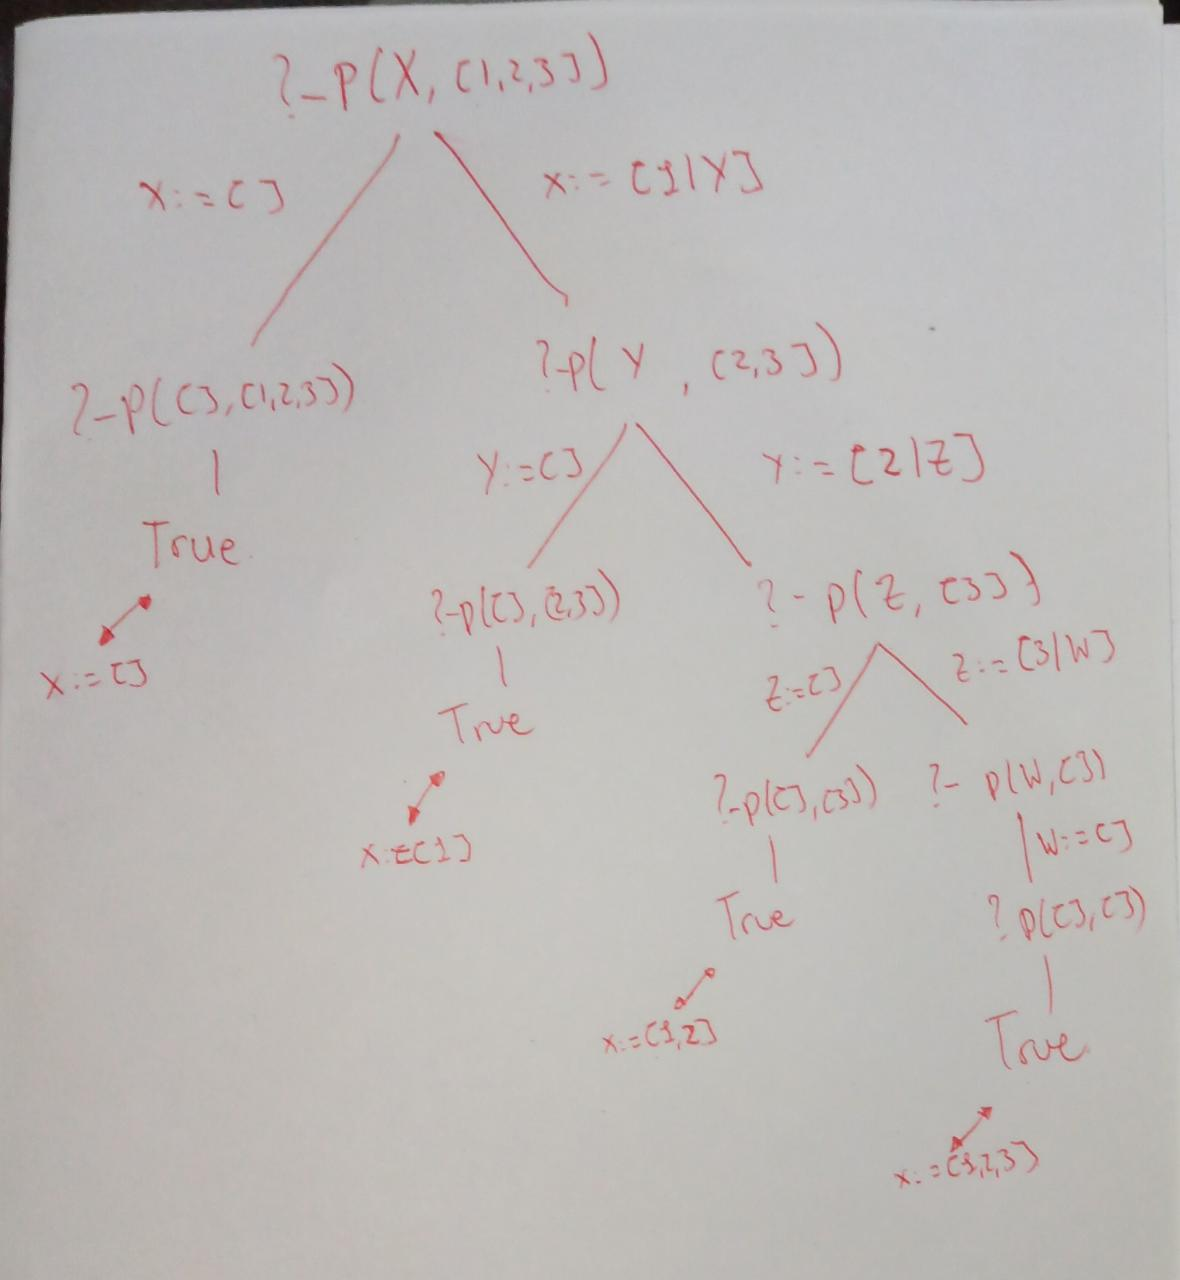
\includegraphics[scale=0.4]{9}
    \end{center}
  \end{enumerate}
\end{enumerate}


\end{document}
